\setlength{\parindent}{0ex}
\setlength{\parskip}{2ex}

\chapter{Coexpression network connectivity affects selection}

\section{Abstract}
The number and strength of interactions between genes will shape the selective effects of mutations in these genes. Specifically, genes with more interactions are likely to be more pleiotropic and will therefore be under stronger constraint and will be less free to adapt. We used coexpression network connectivity in the plant species \textit{Capsella grandiflora} to investigate the relationship between connectivity and selection. Genes with high connectivity have lower amino acid divergence, even when controlling for expression. The relationship between connectivity and divergence appears to be driven by stronger negative selection in highly connected genes. However, positive selection is also stronger in more highly connected genes, implying that positive and negative selection have opposing effects on divergence. Overall, our results show that pleiotropy, as measured through network connectivity, increases selective constraint but does not reduce the adaptive potential of genes.

\section{Introduction}

Variation in quantitative traits results from the combined effects of genetic variation at many genes \citep{lynch1998}, and the ways in which these genes interact can influence how selection shapes this genetic variation. Specifically, genes that have large effects on a specific trait or with pleiotropic effects are likely to be under stronger purifying selection than genes with smaller effects or less pleiotropy\citep{orr2000, stern2008}. Similarly, genes with smaller effects on traits or reduced pleiotropy may be more subject to weaker evolutionary constraint and thus be more free to adapt\citep{orr2000, stern2008}. While these hypotheses are intuitively appealing, we lack still have lack data on how important gene interactions are on a genome-wide scale. One way to estimate the effect size and/or pleiotropy of genes on a genome-wide scale is to use network connectivity information: genes with higher connectivity are more likely to be pleiotropic or large-effect that genes with low connectivity\citep{he2006}. Here, we investigate the relationship between positive and negative selection and network connectivity in the plant \textit{Capsella grandiflora}.

A large body of work has shown that amino acid divergence is affected by network properties, including the number of protein-protein interactions \citep{Fraser2002-rg,Lemos2005-io,Luisi2015-zz} but see \citep{Hahn2004-ke,Jordan2003-ri}, protein-network centrality \cite{Hahn2005-au}, pathway position \citep{Rausher1999-nk,Ramsay2009-vf,Eanes2011-on}, metabolic network connectivity \citep{Vitkup2006-bo}, regulatory network centrality \citep{Jovelin2009-tu}, and coexpression network connectivity \citep{Jordan2004-vj,Carlson2006-ai}. However, reduced amino acid divergence in highly connected genes has been interpreted to be due to either stronger constraint on well-connected genes \citep{Hahn2005-au,Ramsay2009-vf} or more frequent positive selection in genes on the network periphery \citep{Kim2007-xn,Luisi2015-zz}, both of which are possible, but are difficult to distinguish using just divergence-based approaches. In addition, network properties often correlate with expression level, which itself correlates with amino acid divergence, suggesting that expression variation may sometimes underlie observed relationships between amino acid divergence and connectivity \citep{Drummond2006-pa}. However, previous studies have not consistently controlled for the effects of expression on the relationship between connectivity and selection \citep{Jordan2004-vj,Fraser2002-rg}.

Here, we evaluate the relationship between coexpression network connectivity and both positive and negative selection by combining  expression data with information on polymophism and divergence in the plant \textit{Capsella grandiflora}, which has previously been shown to have efficient positive and negative selection \citep{Williamson2014-tf}. We find that connectivity is negatively correlated with amino acid divergence and use polymorphism information to show that this correlation is driven by differences in negative selection: highly connected genes are under stronger negative selection. In addition, we observe stronger positive selection in highly connected genes, suggesting that pleiotropy is not the main factor constraining adaptation across genes of different connectivities. Finally, we observe differences in the strength of positive and negative selection between modules. Collectively, our results suggest that connectivity influences selection on a genome-wide scale.

\section{Results}

We analyzed genome-wide gene expression data from the leaves of 146 \textit{C. grandiflora} individuals from one large population grown in common garden. The expression data from 99 of these individuals has been previously reported \citep{Josephs2015-nx}. For the previously unreported 47 individuals, we generated approximately 1.3 billion single-end RNAseq reads, with a median of 26.7 million reads per individual (range: 19.4 to 44.3 million). Of these, a median of 94.2\% reads mapped to genes (range: 93.1\% to 94.9\%).

\subsection{Coexpression modules}
Twenty-four gene coexpression modules were detected in the \textit{C. grandiflora} expression data using WGCNA \citep{langfelder2008}. These modules ranged in size from 43 to 4,094 genes. Clustering of the module eigengenes revealed that they fell into several broad groups of roughly equal size (Fig.~\ref{fig:fsClust}). Total connectivity values for each gene were calculated as the sum of the connection strengths with all other genes and intramodular connectivity values were calculated as the sum of the connection strengths with the other genes in the same module. These connectivity values show the expected scale-free distribution: there is a linear relationship between the connectivity to a gene (k) and the proportion of nodes with the connectivity (p(k)) when plotted on a log scale (slope = -1.61, r$^{2}$ = 0.96). (Fig.~\ref{fig:fsScale}). This scale free distribution means that most genes have relatively few connections, but some genes have a large number of connections. Total connectivity correlates strongly with intramodular connectivity (correlation coefficient = 0.807), so we chose to focus on intramodular connectivity for the rest of the paper.

Of the 24 \textit{C. grandiflora} coexpression modules detected, eight modules showed a high degree of preservation in \textit{Arabidopsis thaliana}, and another 12 showed a moderate degree of preservation (Table 1). All but one of the modules showed enrichment for GO-process terms that suggest specific biological roles for the different modules (Table 1).

\subsection{Connectivity affects divergence}
Connectivity correlated negatively with  dN ($\rho$ = -0.167, p \textless 0.001,  Fig.~\ref{fig:fsCorr}A), dS ($\rho$ = -0.104, p \textless 0.001, Fig.~\ref{fig:fsCorr}B), and dN/dS ($\rho$ = -0.127, p \textless 0.001) (Fig.~\ref{fig:f1}A). The correlation between dN/dS and connectivity was significant within 7 out of 24 modules (p \textless 0.002), but these were also the largest modules, where there was the most power to detect a correlation (Fig.~\ref{fig:fsMod}). Expression also correlated negatively with dS ($\rho$ = -0.037, p \textless 0.001 Fig.~\ref{fig:fsCorrC}), dN ($\rho$ = -0.276, p \textless 0.001, Fig.~\ref{fig:fsCorr}D), and dN/dS ($\rho$ = -0.261, p \textless 0.001, Fig.~\ref{fig:f1}B),  although the strength of the correlation with dS was quite weak. (Fig.~\ref{fig:fsCorr}). Expression correlates positively with connectivity ($\rho$ = 0.289, p \textless 0.001, Fig.~\ref{fig:f1}C) suggesting that expression variation might explain observed divergence patterns. However, partial correlations that account for expression variation still show a significant although weaker relationship between connectivity and dN ($\rho$ = -0.09, p \textless 0.001), dS ($\rho$ =-0.09, p \textless 0.01) and dN/dS ($\rho$ =-0.05, p \textless 0.001). 

\begin{figure}[ht!]
\centering
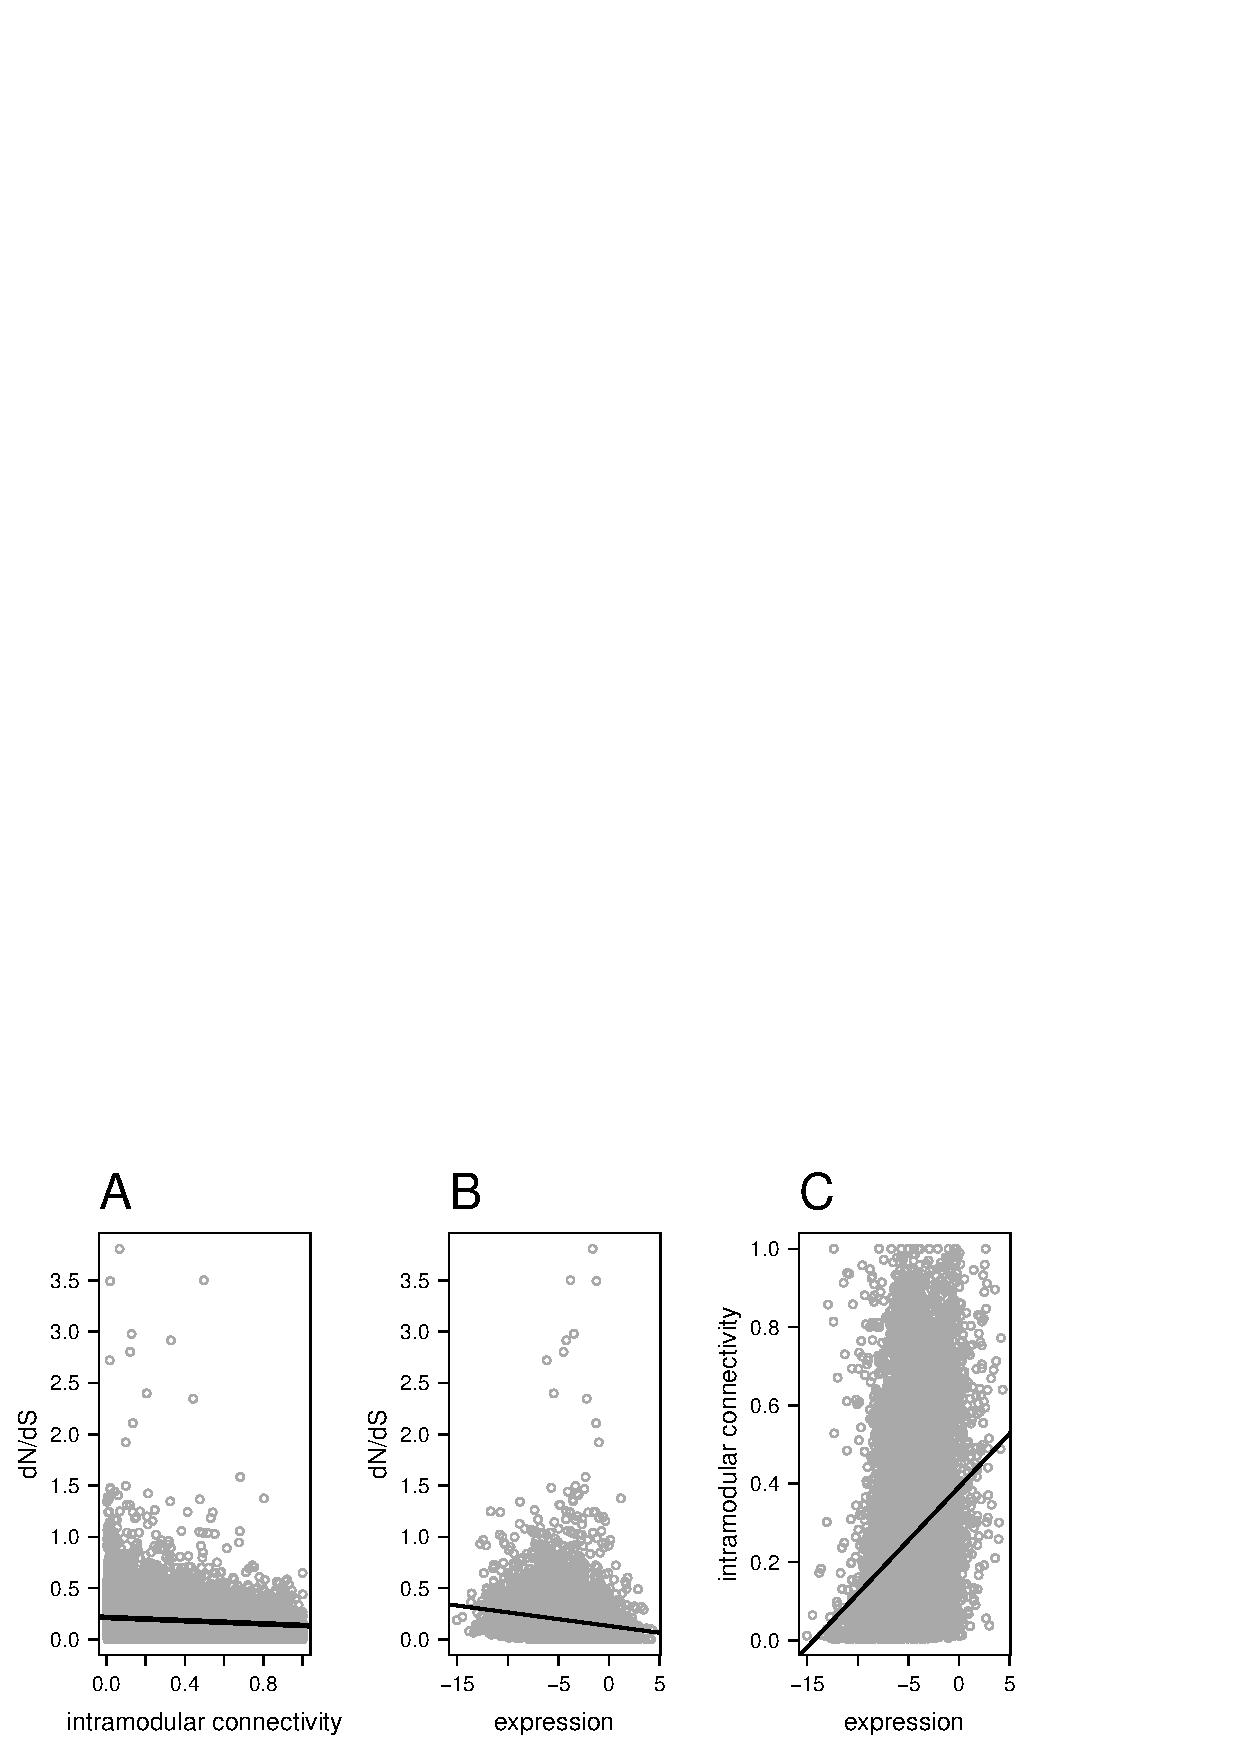
\includegraphics[width=\linewidth]{Ch4Fig1}
\caption{\textbf{Correlations between protein divergence, intramodular connectivity, and expression.} (A) dN/dS correlates negatively with intramodular connectivity ($\rho$ = -0.127, p \textless 0.001). (B) dN/dS correlates negatively with expression ($\rho$ = -0.261, p \textless 0.001). (B) Expression correlates positively with intramodular connectivity ($\rho$ = 0.289, p \textless 0.001)}
\label{fig:f1}
\end{figure}

However, experimental noise in measuring expression can make it difficult to fully remove expression’s effects in a partial correlation, potentially generating spurious correlations \citep{Drummond2006-pa}. To avoid this problem, we followed Drummond et al.’s recommendation and conducted a principal component analysis to identify independent sources of variation in our explanatory variables: dS, expression, intramodular connectivity, and the coefficient of variation in expression (‘expression variaton’). We found that dS and expression variation loaded positively  on PC1, while traits expression level and intramodular connectivity loaded negatively; PC1 explained 32\% of the variation across genes, while PC2, where all explanatory variables loaded negatively, explained 25\% of the variation (Table~\ref{table:t2}). A linear model based on the four principal components and all possible interactions explained $\sim$ 22\% of the variation in dN (Table~\ref{table:t2}). The first principal component explained 14\% of the variation in dN and was determined by all four explanatory variables, suggesting that dS and expression variation contribute positively to dN while intramodular connectivity and expression level contribute negatively to dN. 

\begin{table}[ht!]
\centering
\begin{tabular} {|l|l l l l l|}
\hline
 &PC1 &PC2 &PC3 &PC4 &All \\ [0.5ex]
\hline
\% variation in dN explained & 13.75 &2.23 &0.98& 1.34 & 21.67\\
P value & 0 & 1.5x10$^{-82}$ & 2.0x10$^{-37}$ & 1.2x10$^{-50}$ &  \\
Direction of effect & + & - & + & - & \\
\% of variance explained & 32.9 &25.5 &21.5 &20.6 &100\\
\hline
Contributions to PCs & & & & & \\ [0.5ex]
dS & 0.512 & -0.481 & 0.420 & 0.566 & \\
Expression level & -0.539 &-0.332 &0.702 & -0.328 & \\
Expression variation &0.573 &-0.328 &-0.065 &-0.748 & \\
Intramodular connectivity &-0.344 &-0.742 &-0.564 &0.110 & \\
\hline
\end{tabular}
\caption{\textbf{Parameters and results from principal components analysis}}
\label{table:t2}
\end{table}

\subsection{Connectivity affects positive and negative selection}
Reduced divergence in highly connected genes could be caused either by stronger negative selection or weaker positive selection. To investigate these alternatives, we divided all genes that were expressed in \textit{C. grandiflora} leaf tissue into four equally-sized categories based on intramodular connectivity and estimated the proportion of 0-fold degenerate sites in these categories under various strengths of purifying selection \citep{Eyre-Walker2009-zt}.

The strength of negative selection across all expressed genes was similar to those observed in a previous study of a species-wide sample of \textit{C. grandiflora} (Fig.~\ref{fig:fsAll}A). However, $\alpha$ (the proportion of all 0-fold degenerate fixations due to positive selection) and $\omega$ (the rate of 0-fold degenerate fixations due to positive selection) were somewhat lower than observed in the species-wide sample: $\alpha$ in the population sample was 0.32 compared to 0.41 in the species-wide sample and $\omega$ was 0.06 compared to 0.08 in the species-wide sample (Fig.~\ref{fig:fsAll}B, C) \citep{Williamson2014-tf}.

In general, negative selection acted more strongly on genes with higher connectivity (Fig. ~\ref{fig:f2}). For example, 0.193 (95\% CIs: 0.186 - 0.197) of 0-fold degenerate sites in genes in the lowest connectivity category are effectively neutral (\textit{N$_{e}$S} \textless 1) while 0.115 (95\% CIs: 0.112 - 0.127) of 0-fold degenerate sites in genes in the highest connectivity category have \textit{N$_{e}$S} \textless 1 (p \textless 0.01)(Fig. ~\ref{fig:f2}A). Positive selection also acted more strongly in highly connected genes. $\alpha$, was 0.209 (95\%CIs: 0.295 - 0.476) in the lowest connectivity category and 0.455 (95\% CIs: 0.395-0.476) in the highest connectivity category (p \textless 0.01)(Fig. ~\ref{fig:f2}B). $\omega$ was also higher in highly connected genes (0.0834, 95\% CIs: 0.0722-0.0895) than genes with low connectivity (0.0449, 95\%CIs: 0.00740-0.0594) (p \textless 0.005)(Fig. ~\ref{fig:f2}C).

\begin{figure}[ht!]
\centering
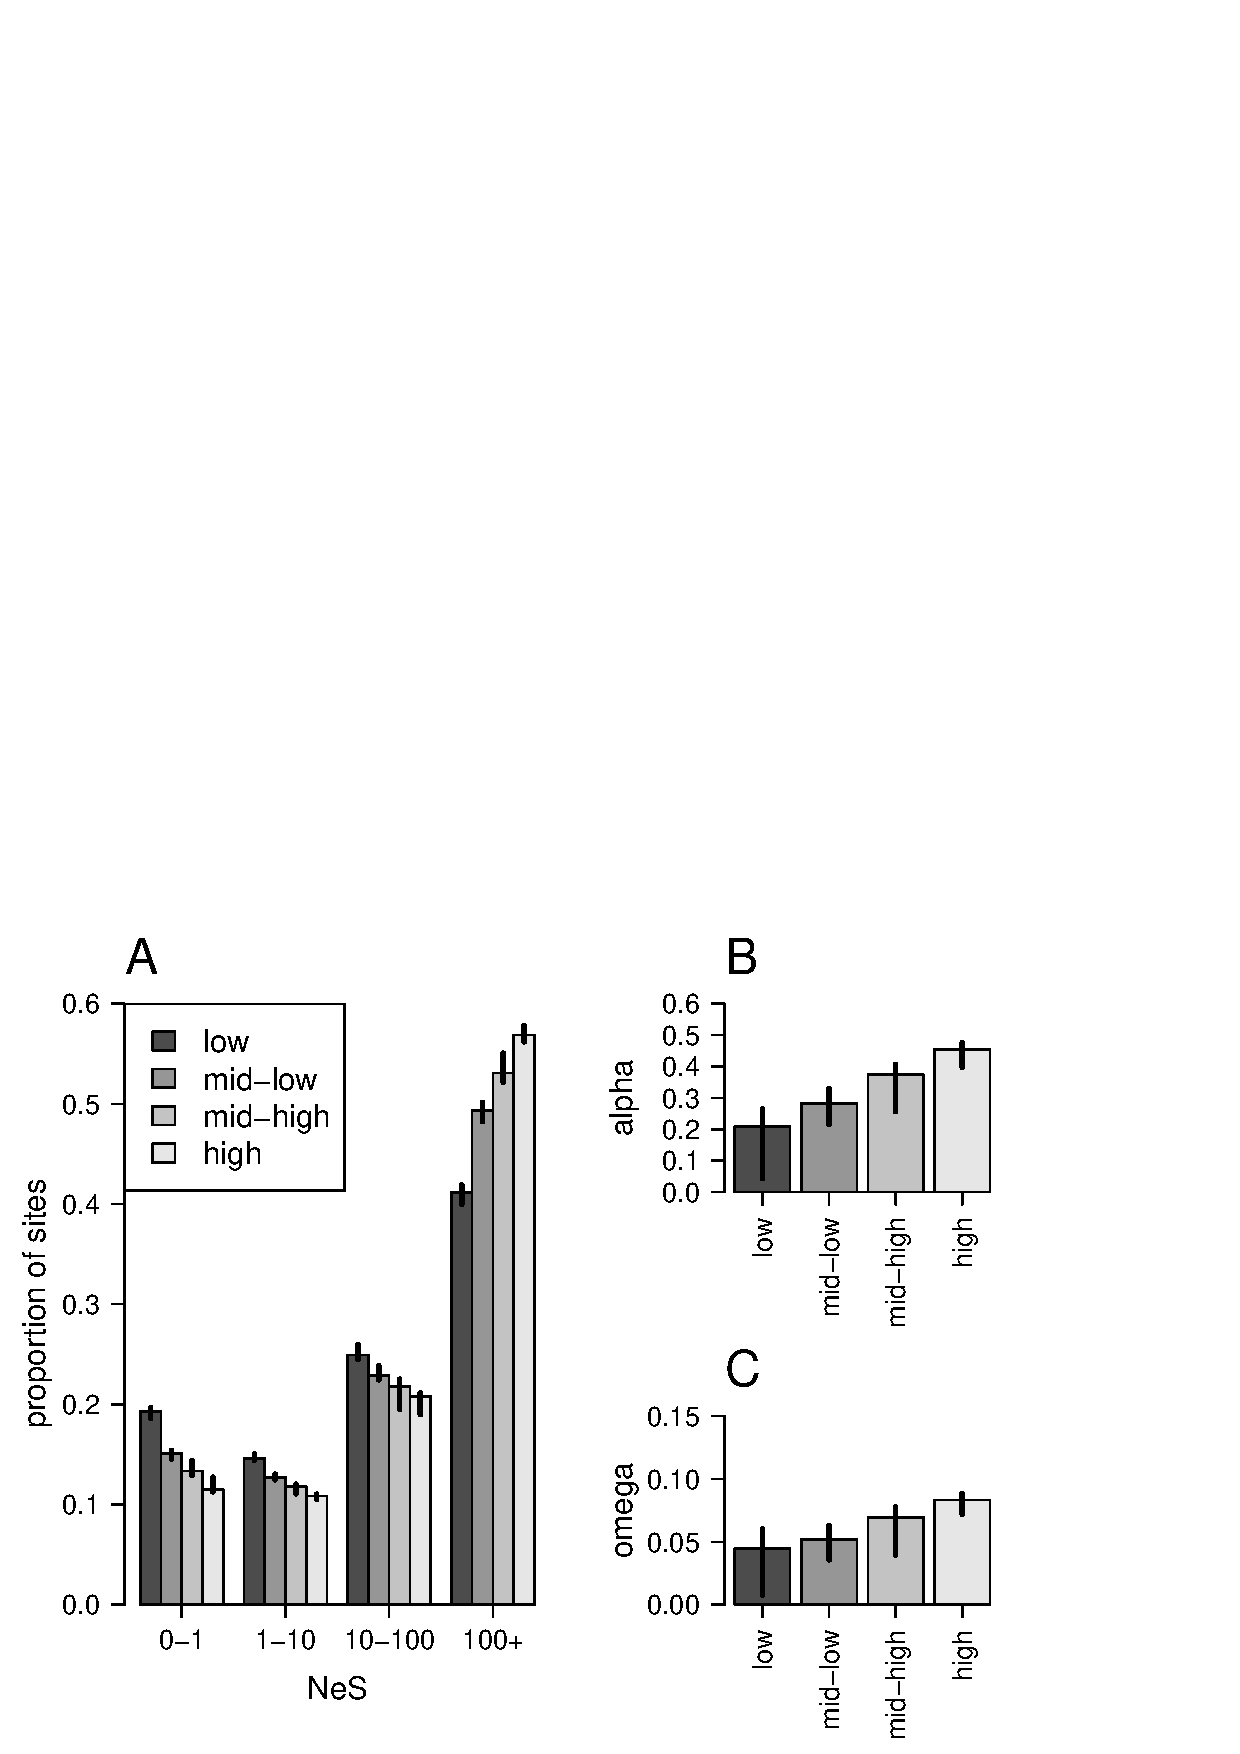
\includegraphics[width=\linewidth]{Ch4Fig2}
\caption{\textbf{ Estimates of negative and positive selection in genes of different connectivity categories.} A) The proportion of sites found in each bin of purifying selection strength, separated by connectivity category. B) The proportion of sites fixed by positive selection, and C) the rate of adaptive substitution. Error bars represent 95\% confidence intervals.}
\label{fig:f2}
\end{figure}

However, expression level could also explain stronger negative selection in highly connected genes, since expression level is correlated with connectivity and genes with higher expression in leaf tissue in \textit{C. grandiflora} experience stronger negative selection \citep{Williamson2014-tf}. To control for expression level in this analysis, we found a subset of our dataset within a narrow range of expression levels where expression level and connectivity were not correlated and repeated our analysis of selection on this subset of genes (N = 2,714). Within this subset, negative selection was still stronger on genes with higher connectivity values, although this effect was somewhat weaker: 0.113 (95\% CIs: 0.100 - 0.129) of sites in the lowest connectivity category were effectively neutral (\textit{N$_{e}$S} \textless 1) while only 0.08 (95\% CIs: 0.0741-0.0882) of 0-fold degenerate sites in the highest connectivity category were neutral (p \textless 0.01) (Fig. ~\ref{fig:f3}A). 

Since no relationship between the rate of positive fixations ($\omega$) and expression has been observed \citep{Williamson2014-tf}, it seems likely that the differences in $\omega$ observed between connectivity classes in the entire dataset are free of the confounding effects of expression. However, we still investigated positive selection in our subset and found that positive selection was stronger on highly connected genes, although reduced sample size made it difficult to calculate measures of positive selection for the lowest connectivity category, which had only 251 genes. Still, the trend suggests that positive selection is stronger in highly connected genes. $\alpha$ is 0.433 (95\% CIs: 0.371 - 0.510) in genes in the highest connectivity class and 0.324 (95\% CIs: 0.182 - 0.411) in the mid-low connectivity category (p \textless 0.05) (Fig.~\ref{fig:f3}B). Similarly, $\omega$ was higher in the highest connectivity class (0.0557, 95\% CIs: 0.0443-0.0682) than in the mid-low connectivity class (0.0413, 95\% CIs: 0.0191-0.0585, p = 0.19)(Fig.~\ref{fig:f3}C). 


\begin{figure}[ht!]
\centering
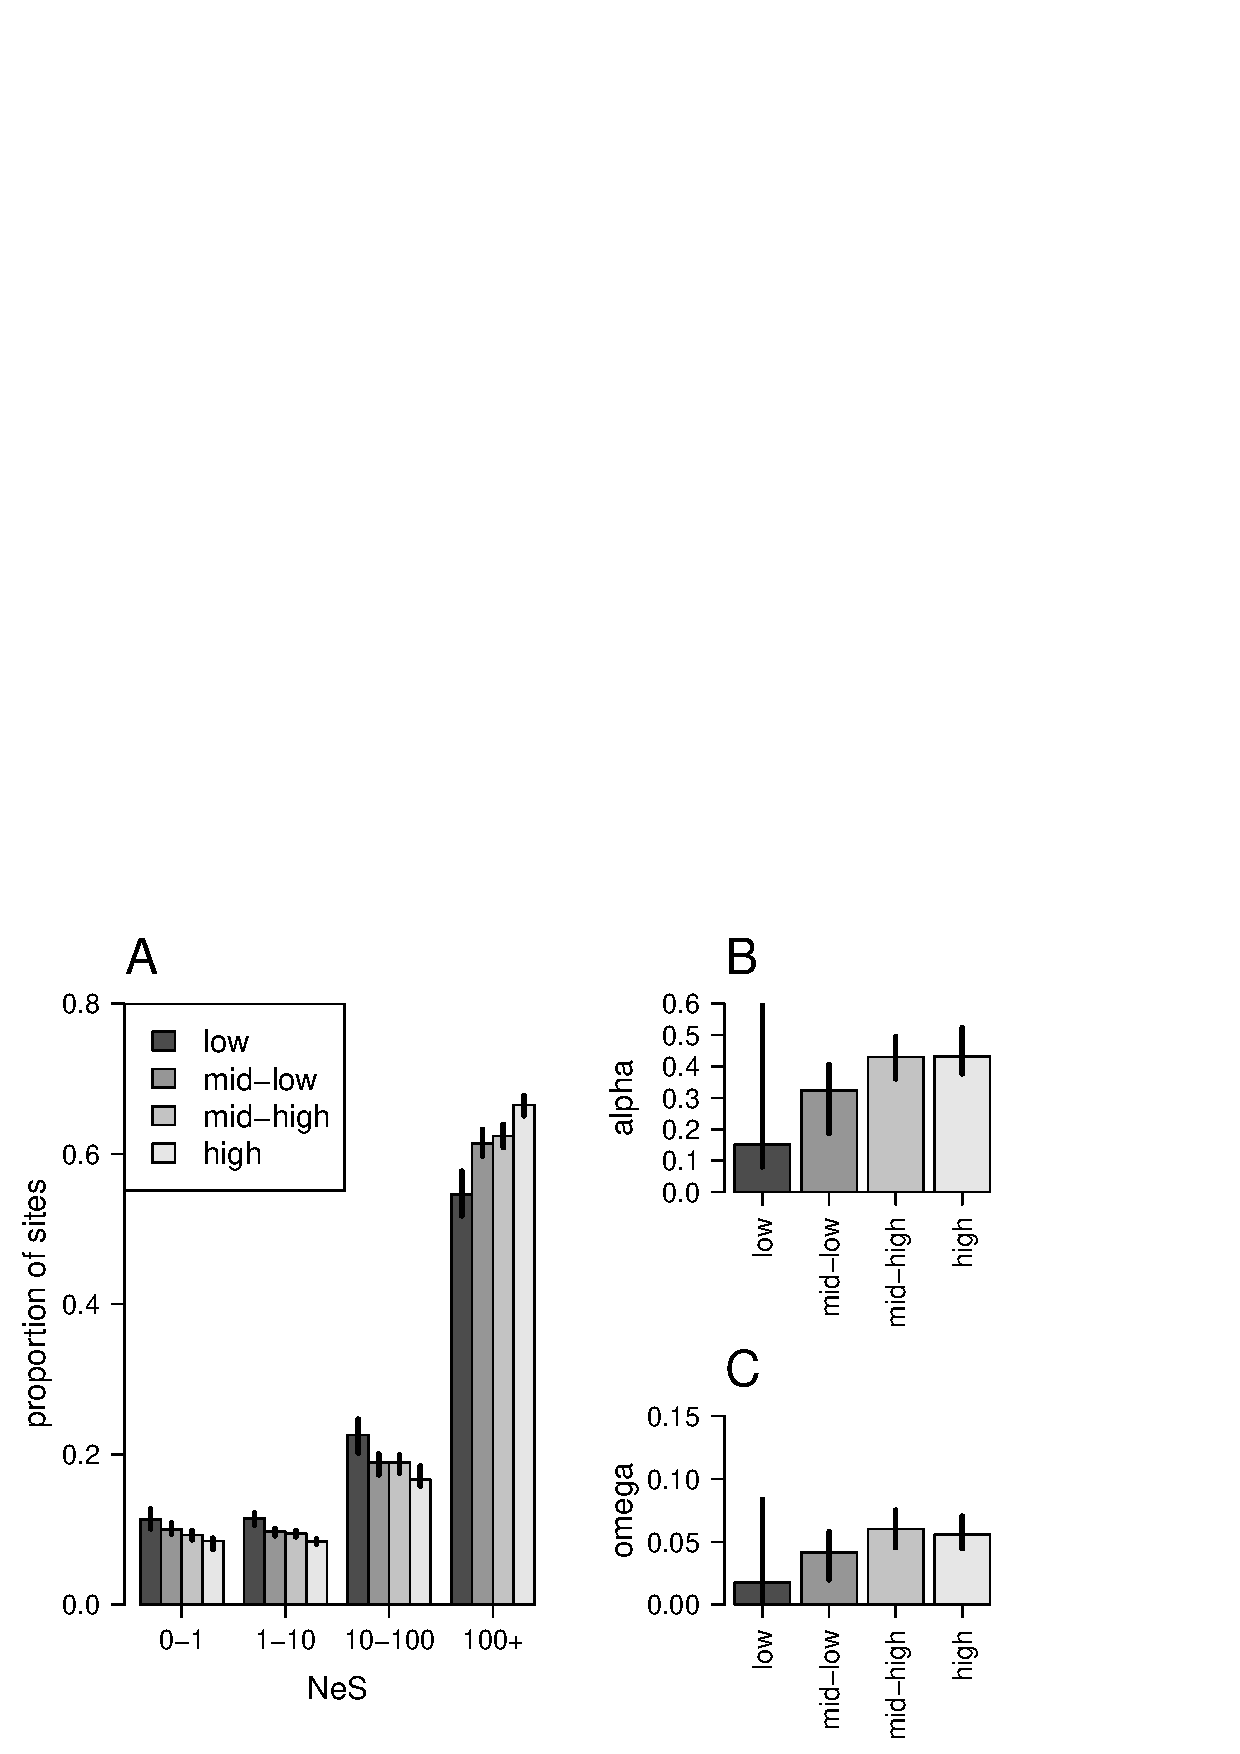
\includegraphics[width=\linewidth]{Ch4Fig3}
\caption{\textbf{Estimates of negative and positive selection in genes of different connectivity categories within the subset where expression does not correlate with connectivity.} A) The proportion of sites found in each bin of purifying selection strength, separated by connectivity category. B) The proportion of sites fixed by positive selection, and C) the rate of adaptive substitution. Error bars represent 95\% confidence intervals.}
\label{fig:f3}
\end{figure}


\subsection{Selection across coexpression modules}
The strength of positive and negative selection varies across modules (Fig.~\ref{fig:f4}). The proportion of 0-fold degenerate sites evolving neutrally (\textit{N$_{e}$S} \textless 1) ranged from 0.102 (grey60) to 0.216 (skyblue3) (Fig.~\ref{fig:f4}A). The proportion of 0-fold degenerate fixations due to positive selection within modules ranged from  0.412 (skyblue3) to 0.531 (yellowgreen) and the rate of 0-fold degenerate fixation due to positive selection ranged from 0.025 (magenta) to 0.145 (yellowgreen) (Fig.~\ref{fig:f4}B). There was no correlation between the proportion of 0-fold degenerate sites in a module that evolve neutrally (\textit{N$_{e}$S} \textless 1) and the rate of fixation due to positive selection ($\omega$). (Pearson correlation, p = 0.34). 

We investigated the GO processes enriched in modules that experience the strongest positive selection to get a better picture of what biological processes may be under selection in our population. The module that experiences the strongest positive selection (yellowgreen, $\alpha$ = 0.531, $\omega$ = 0.147) had a number of enrichments for GO processes, including response to chitin, response to organonitrogen compound, response to nitrogen compound, and a number of processes involved in defense response and immune systems. (Table 1). The module with the second highest $\alpha$ and third highest $\omega$ (lightsteelblue1, $\alpha$=0.517, $\omega$ = 0.103) also had enrichments in defense related genes. (Table 1).  The module with the second highest $\omega$ (0.1046) and seventh highest $\alpha$ (0.403), saddlebrown, had enrichments in processes involved in DNA replication and epigenetic regulation of gene expression.

For the most part, modules under weak positive selection had enrichments in different modules than those under strong positive selection. For example, the magenta module ($\alpha$ = 0.166, $\omega$ = 0.025) had enrichments in phosphalitidylinositol biosenthetic and metabolic processes, but the darkgrey module ($\alpha$=0.182, $\omega$ = 0.027) did not have any significant enrichments. The midnightblue module, with the third lowest measures of positive selection ($\alpha$ = 0.189, $\omega$=0.030 ) had enrichments in response to chitin, organonitrogen compounds, and nitrogen compounds. The surprising result that both a module under the strong positive selection (yellowgreen) and a module under weak positive selection (midnightblue) share similar GO processes suggests that not all the genes in this GO process are under the same selective pressures and that coexpression analysis was able to separate genes by selective pressure.


\begin{figure}[ht!]
\centering
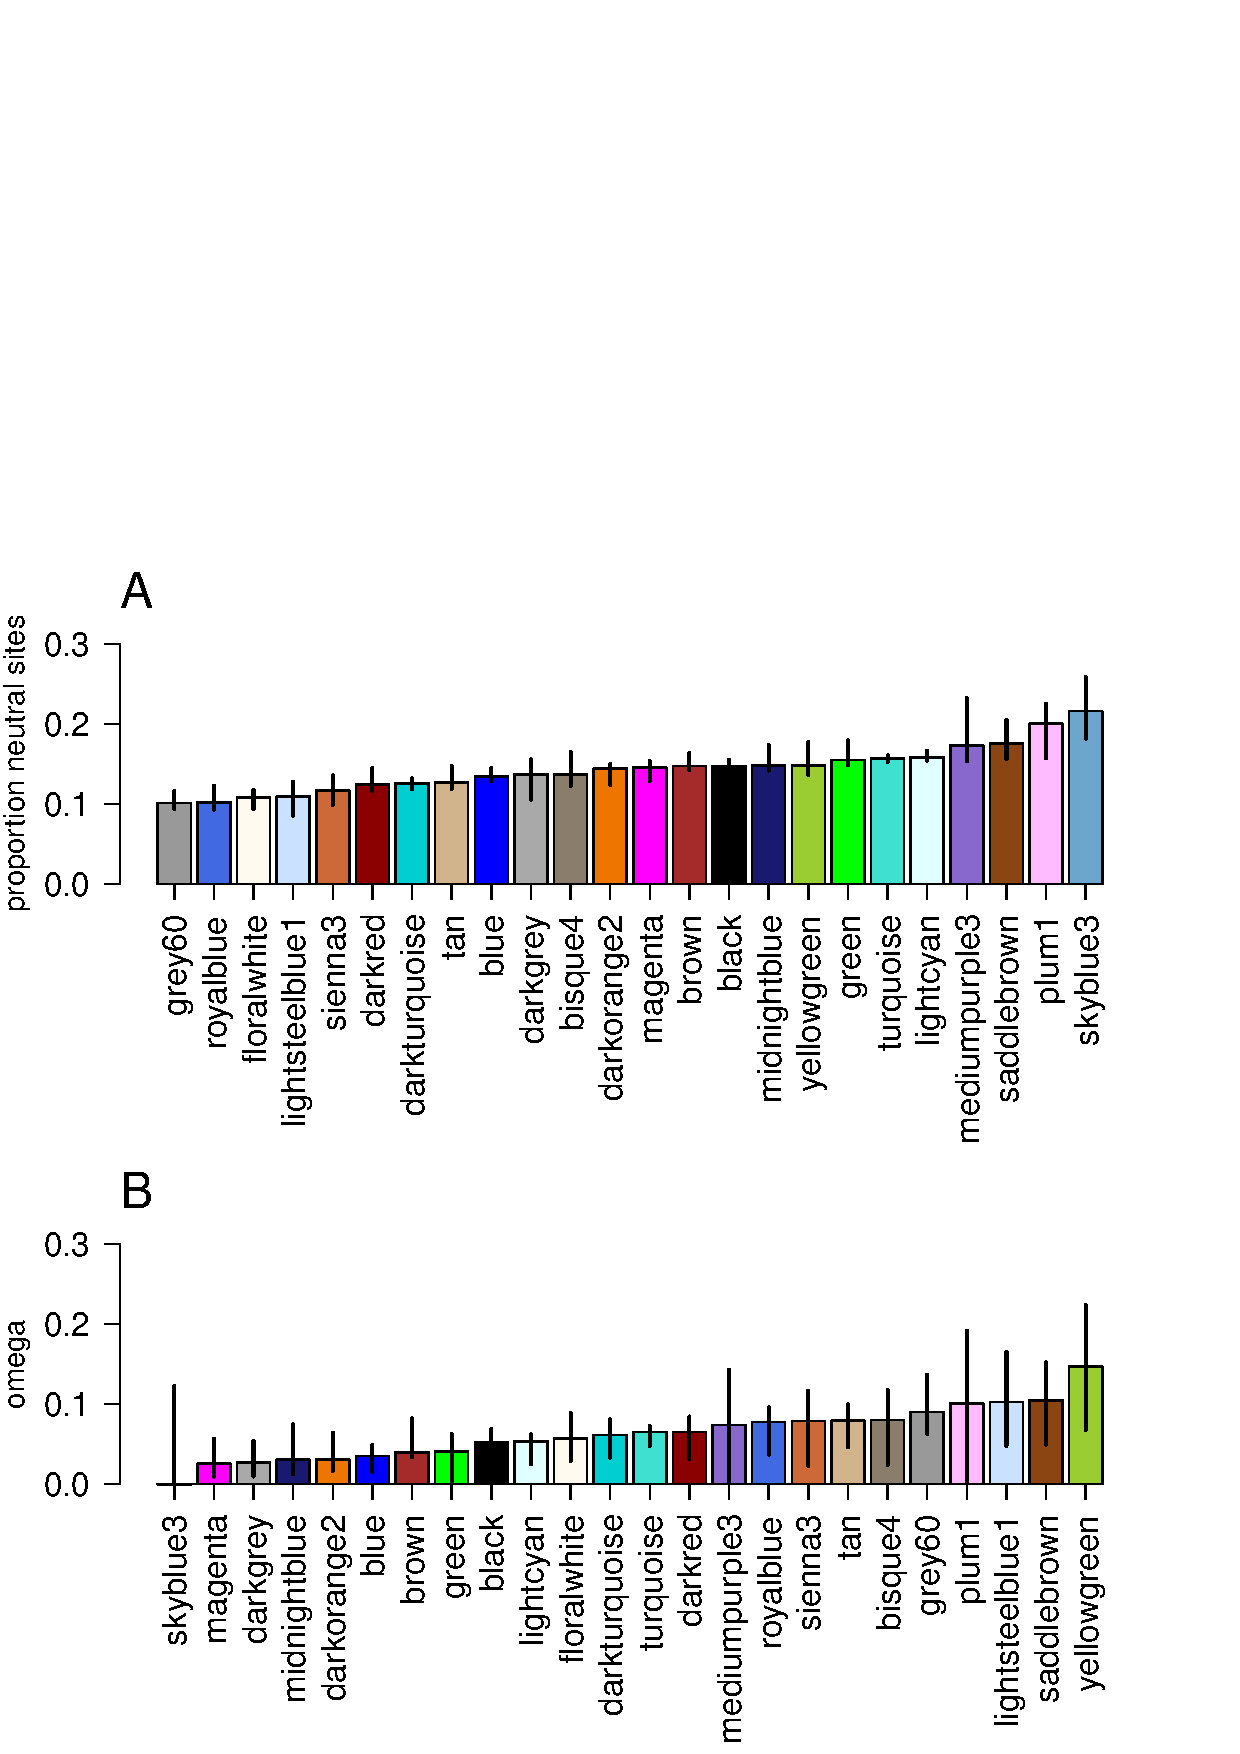
\includegraphics[width=\linewidth]{Ch4Fig4}
\caption{\textbf{Positive selection across modules.} A) shows the proportion of sites where NeS < 1 across modules. Black bars represent 95\% confidence intervals. B) shows $\omega$ across modules. Black bars also represent 95\% confidence intervals.
}
\label{fig:f4}
\end{figure}


\section{Discussion}

In this study we investigated the relationship between connectivity and other coexpression network properties and selection in the plant \textit{C. grandiflora}. Intramodular connectivity was negatively associated with dN/dS, suggesting that constraint is stronger on highly connected genes. However, when we analyzed positive and negative selection separately, we found that connectivity increases the strength of both negative and positive selection. Finally, there were significant differences in the strength of selection between coexpression modules.

Most previous work on the relationship between connectivity and selection has focused on amino acid divergence, making it difficult to separate the effects of positive and negative selection. However, by using polymorphism to investigate the distribution of fitness effects and, then, an extension of the McDonald-Kreitman test to estimate positive selection, we were able to detect positive selection and negative selection which would have opposite effects on divergence. One other study that investigated positive selection’s relationship to network centrality also ran into difficulties separating the effects of negative and positive selection on divergence. \citep{Luisi2015-zz} used human data to detect a positive relationship between network degree and signatures of linked selection on neutral polymorphisms but they found a negative relationship between network centrality and estimates of positive selection based on divergence.. Our results suggest that previous studies that did detect an effect of connectivity on protein divergence may be underestimating the effect of connectivity on negative selection and entirely missing the effect of connectivity on positive selection because of these forces’ conflicting effects on divergence.

We are not the first to note a relationship between connectivity and synonymous divergence \citep{Jordan2004-vj}. The cause of this correlation seems unclear. Jordan et al. suggested that highly connected genes may have have more constraint on synonymous sites due to translational regulation. A full understanding of the causes of the relationship between connectivity and dS will likely depend on developing a better picture of the mechanism driving the relationship between connectivity and other selective parameters.

A relationship between positive and negative selection and coexpression network connectivity could result from a few different biological mechanisms. First, genes with higher connectivity could have more pleiotropic effects \citep{he2006}, which would constrain sequence evolution. However, while it has been suggested that highly pleiotropic genes should experience reduced positive selection \citep{orr2000, stern2008}, we do not observe this in our data. Alternatively, mutations in genes with higher connectivity may have larger phenotypic effect sizes, suggesting that both positive and negative selection may be stronger in highly connected genes \citep{Olson-Manning2012-ap}. This latter hypothesis better fits our own findings that positive selection is stronger in well-connected genes.

Linking the relationship between connectivity and selection to a specific biological mechanism will require a closer understanding of how coexpression connectivity relates to pathway and network structure. A number of studies have investigated pathway position and selection in specific pathways. For example, genes in the human innate immune system are more constrained when they have many connections with other genes while genes at the top and the bottom of the network have the strongest evidence of positive selection \citep{Casals2011-jz}. However, the insulin and target of rapamycin pathways show opposite patterns (reviewed in \citep{Olson-Manning2013-op}. However, there is no clear way to link coexpression network connectivity with directionality and pathway structure, making it difficult to evaluate specific predictions about network structure with coexpression networks.

Observations that the evolutionary rate varies between genes were initially hypothesized to be due to variation in the proportion of gene sites under constraint: genes with a larger portion of constrained sites evolved slowly. (\citep{Kimura1977-ib}). This view implies that variation in evolutionary rates relates directly to the function of the proteins. However, later investigations suggested that most or even all of the variation in evolutionary rates between proteins was not due to function at all, but instead a by-product of expression level variation that makes deleterious mutations more deleterious in highly expressed genes. \citep{Drummond2006-pa,Zhang2015-ne}. While it is undeniable that expression level does influence evolutionary rates, by demonstrating a relationship between connectivity and both negative and positive selection, we have shown that protein function does contribute to the variation in selection between genes, suggesting that gene function matters on a genome-wide scale for determining genetic variation. 


\section{Materials and Methods}

\subsection{Measuring expression}
We used leaf expression data from a population sample of 99 individuals of \textit{C. grandiflora} reported in \citet{Josephs2015-nx} and an additional 48 individuals, first reported here. All 147 individuals descend from the same population collected near Monodendri in Greece, were grown in the same growth chamber, and underwent the same tissue collection and RNA extraction procedure, described in \citet{Josephs2015-nx}. The RNA from the previously unreported 48 individuals was sequenced at the Genome Quebec Innovation Centre in an Illumina HiSeq in one flow cell with 7 or 8 samples per lane (additional samples were sequenced and but were not included in this analysis). All reads from these 48 individuals were 100bp long and single ended. The first 99 individuals were sequenced paired-end in 100bp long reads, so to avoid the confounding effects of mapping accuracy, we randomly selected one read per pair for further analysis.

All sequence data was mapped using Stampy 1.0.21 \citep{Lunter2011-uc} with default settings to an exon-only reference \citep{Josephs2015-nx}. We measured expression level for each gene by counting the number of reads that mapped to each gene using the HTSeq.scripts.count feature from HTSeq and we normalized for sequencing depth by dividing by the median expression level for each individual \citep{Anders2015-qa}. We did not detect interactions between GC content, expression level, and lane \citep{Josephs2015-nx}. Genes with a median expression of 0 were removed from the analysis, leaving a total of 20,570 genes. For comparisons of expression level and divergence and selection we divided read count by gene length, measured as the number of nucleotides in the coding sequence, to make expression level comparable between genes.

\subsection{Construction of Capsella grandiflora gene co-expression network}
The R package, WGCNA version 1.34, running under R version 2.15.1 \citep{r} was employed to construct gene coexpression networks for the \textit{C. grandiflora} expression data \citep{langfelder2008}. This type of analysis groups together genes with similar patterns of pairwise correlation of expression, patterns that in theory are expected to reflect a shared role within similar biologically meaningful functional pathways and processes. We were interested in retaining the information embodied in the sign of the gene expression correlations, so we conducted a signed network analysis using the following adjacency function: a$_{ij}$ = |0.5 + 0.5 x cor(x$_{i}$,x$_{j}$)|, where cor(x$_{i}$,x$_{j}$) is the correlation of gene expression of the i$^{th}$ and j$^{th}$ gene, and is the soft thresholding value. Soft thresholding is used in WGCNA, as it typically leads to co-expression networks that exhibit a scale-free degree distribution pattern of node connectivity, an inherent property of biological networks. 

The \textit{C. grandiflora} gene co-expression networks were obtained using  a soft thresholding power of 12, as suggested by the authors of the WGCNA package for signed networks. Genes that exhibited similar patterns of connectivity (i.e., genes showing high “topological overlap”) were grouped together in the same coexpression modules, based on hierarchical clustering of topological overlap values, in which a dynamic branch-cutting algorithm was used to define initial gene co-expression modules \citep{langfelder2008}.  Module eigengenes (the first principal component of the gene expression values of modules) were calculated and modules whose eigengenes were highly correlated were merged to arrive at the final set of co-expression modules. The resulting modules were labeled with different colors for ease of referencing. A preliminary coexpression analysis showed that one individual was a strong outlier, so we removed it and reran the analysis on the remaining 146 individuals. Total connectivity for each gene was calculated as the sum of connection strengths between the focal gene and all other genes and intramodular connectivity was calculated as the sum of connections between the focal gene and all other genes in the same module. 

\subsection{Co-expression module preservation analysis}
Module preservation analysis aims to determine whether and to what extent co-expression modules detected in one data set (the “reference data set”) are conserved in a second (or “test”) data set. The reference gene co-expression modules and data set in this case were from the \textit{C. grandiflora} gene expression data and analysis described above, while the test data were from RNAseq reads for 19,706 genes obtained from RNA collected from seedling tissue of 20 ecotypes of \textit{A. thaliana}, obtained from published data \textit{Gan2011-xv}. Module preservation analysis does not require network construction for the test data set. Instead, the module assignment based on analysis of the reference (\textit{C. grandiflora}) set is applied to the test (\textit{A. thaliana}) set, and network-based preservation statistics are calculated and combined into a single composite preservation measure that reflects preservation of both module density and module connectivity patterns \citep{langfelder2011}. By randomly permuting the module labels assigned to the test data and re-calculating the network-based preservation statistics n times (n = 200 times for the analyses reported here), one can calculate a Z-statistic for the composite preservation measure associated with each reference module, referred to here as a Z-summary statistic.  The Z-summary statistic asymptotically follows the normal distribution with mean 0 and SD = 1, and can be converted to a p-value under the standard normal distribution.  Simulations conducted by Langfelder et al. (2011) show that Z-summary values > 10 correspond with strong evidence of module preservation in the test data, Z-summary values between 2 and 10 correspond with moderate evidence of module preservation in the test data.

\subsection{GO enrichment analysis of genes in modules}
We used the GOrilla software package to search for GO terms enriched in the \textit{A. thaliana} orthologs (from \citep{Williamson2014-tf}) of each co-expression module \citep{Eden2009-hl}. 16,672 of our expressed genes had \textit{A. thaliana}, though GOrilla had GO terms for only 10,079 of these genes, and so the enrichment analysis is based on this subset.

\subsection{Measuring divergence}
Divergence measurements from each gene were previously published in \citep{Williamson2014-tf} and detailed methods are included there. Briefly, we found orthologs between the \textit{Capsella rubella} reference genome and its two closest outgroups: \textit{Neslia paniculata} and \textit{A. thaliana} and aligned the protein sequences of these orthologs. These alignments were used to calculate dN and dS using codeml in PAML in a model where divergence was allowed to vary in the lineage leading to \textit{C. rubella} \citep{Yang2007-rs}. Nine genes with zero synonymous substitutions were removed from the analysis so that dN/dS could be calculated.

\subsection{Relating divergence to connectivity and other parameters}
We conducted Spearman correlations between connectivity and divergence and connectivity and expression for each gene (N=13,211) using R’s cor.test() function \citep{r}. Partial Spearman correlations between connectivity and divergence while accounting for expression were conducted with the pcor.test() function from the ppcor library in R. A principal component analysis for dS, mean expression level, the coefficient of variation for expression level, and intramodular connectivity was conducted in R using the prcomp() function, with scaling. We also used the R lm() function to construct a linear model for how principal components predict variation in dN.

\subsection{Measuring selection}
The strength of positive and negative selection in the \textit{C. grandiflora} genome was measured using single nucleotide polymorphism (SNP) data from 178 individuals collected from the same population described above and previously reported in \citep{Josephs2015-nx,Sicard2015-uc}. 146 of these 178 individuals overlap with the individuals used to generate coexpression networks.

DNA was extracted by either a CTAB based protocol or by DNeasy Plant Mini Kit (Qiagen). We obtained whole genome sequences from each individual through 100 cycles of paired end sequencing in a Hiseq 2000 with Truseq libraries (Illumina) and three individuals were sequenced per lane. We subsequently followed GATK Best Practices for Variant Quality Recalibration circa GATK 2.7 \citep{DePristo2011-jc} using a high confidence “truth” set generated by filtering SNPs for concordance with common variants (\textless0.11) in a species-wide sample of \textit{C. grandiflora} as well as suspect realignments (transposable elements, centromeres, 600 bp intervals containing extreme Hardy Weinberg deviations, 1 kb intervals that showed evidence of three or more SNPs in a reference-to-reference mapping of 150 bp paired end reads from the reference genome line). Inter-relatedness among lines was < 5\%. For population genetic analysis, we downsampled to 320 alleles by randomly classifying alleles as missing, which allowed retention of 94.2\% of sites.

Divergence was measured from an outgroup, \textit{Neslia paniculata}, aligned to \textit{C. rubella} using LastZ with chaining, as described in \citep{Haudry2013-qe}. We used the Joint Genome Institute’s gene annotation of the \textit{C. rubella} reference genome to identify 0-fold degenerate and 4-fold degenerate sites within genes. We assigned these genes into categories based on kWithin values and coexpression module membership and calculated site frequency spectra (SFS) and divergence at 0-fold degenerate and 4-fold degenerate sites within these categories.  We used SFS and divergence to estimate the fraction of 0-fold degenerate sites within each category under negative selection and $\alpha$ using DFE-$\alpha$, using 4-fold sites as a neutral reference \citep{eyre2009,keightley2007}. 200 bootstraps were conducted by resampling the genes included within each category with replacement. We used these bootstraps to construct 95\% confidence intervals and we generated two-tailed p-values by calculating the proportion of bootstraps where selection was higher in the less selected category than the more selected category and multiplying by two \citep{Eyre-Walker2009-zt}. 



\section{Acknowledgements}
Robert Williamson, Adrian Platts, Wei Wang, Alan Moses, Asher Cutter.

\section{Appendix: Supplementary figures and tables}

\begin{landscape}

\begin{table}[ht]
\centering
\begin{tabular}{|l|rrrrrlP{5cm}r|}
  \hline
Module & Z & N & \textit{N$_{e}$S} \textless 1 & $\alpha$ & $\omega$ & GO Term & Description & p \\ 
  \hline
bisque4 & 3.827 & 191 & 0.137 & 0.402 & 0.080 & GO:0010207 & photosystem II assembly & 1.9E-09 \\ 
   &  &  &  &  &  & GO:0019252 & starch biosynthetic process & 6.1E-08 \\ 
   &  &  &  &  &  & GO:0005982 & starch metabolic process & 1.2E-07 \\ 
   &  &  &  &  &  & GO:0000023 & maltose metabolic process & 1.6E-07 \\ 
   &  &  &  &  &  & GO:0005984 & disaccharide metabolic process & 6.4E-07 \\ 
\hline
  black & 8.104 & 1106 & 0.147 & 0.290 & 0.053 & GO:1902589 & single-organism organelle organization & 4.3E-05 \\ 
   &  &  &  &  &  & GO:0022402 & cell cycle process & 4.5E-05 \\ 
   &  &  &  &  &  & GO:0009630 & gravitropism & 8.9E-05 \\ 
   &  &  &  &  &  & GO:0009606 & tropism & 8.9E-05 \\ 
   &  &  &  &  &  & GO:0009629 & response to gravity & 1.4E-04 \\ 
\hline  
blue & 12.664 & 2066 & 0.134 & 0.230 & 0.035 & GO:0043043 & peptide biosynthetic process & 1.6E-90 \\ 
   &  &  &  &  &  & GO:0006412 & translation & 3.8E-90 \\ 
   &  &  &  &  &  & GO:0043604 & amide biosynthetic process & 6.0E-87 \\ 
   &  &  &  &  &  & GO:0006518 & peptide metabolic process & 4.2E-86 \\ 
   &  &  &  &  &  & GO:0043603 & cellular amide metabolic process & 7.8E-77 \\ 
\hline  
brown & -1.149 & 2757 & 0.147 & 0.236 & 0.040 & GO:0006914 & autophagy & 1.2E-09 \\ 
   &  &  &  &  &  & GO:0044248 & cellular catabolic process & 6.9E-07 \\ 
   &  &  &  &  &  & GO:0046700 & heterocycle catabolic process & 1.5E-04 \\ 
   &  &  &  &  &  & GO:0044242 & cellular lipid catabolic process & 1.7E-04 \\ 
   &  &  &  &  &  & GO:0019439 & aromatic compound catabolic process & 2.2E-04 \\ 
\hline 
 darkgrey & 1.195 & 357 & 0.137 & 0.182 & 0.027 &  NA &  NA & NA \\ 
\hline
  darkorange2 & 4.598 & 982 & 0.144 & 0.196 & 0.031 & GO:0010264 & myo-inositol hexakisphosphate biosynthetic process & 2.5E-05 \\ 
   &  &  &  &  &  & GO:0033517 & myo-inositol hexakisphosphate metabolic process & 2.5E-05 \\ 
   &  &  &  &  &  & GO:0032958 & inositol phosphate biosynthetic process & 4.0E-05 \\ 
   &  &  &  &  &  & GO:0046173 & polyol biosynthetic process & 6.3E-05 \\ 
   &  &  &  &  &  & GO:0043647 & inositol phosphate metabolic process & 3.4E-04 \\ 
\hline
\end{tabular}
\end{table}


\begin{table}[ht]
\centering
\begin{tabular}{|l|rrrrrlP{5cm}r|}
  \hline
Module & Z & N & \textit{N$_{e}$S} \textless 1& $\alpha$ & $\omega$ & GO Term & Description & p \\ 
  \hline
  darkred & 3.277 & 456 & 0.124 & 0.375 & 0.065 & GO:0048583 & regulation of response to stimulus & 2.0E-05 \\ 
   &  &  &  &  &  & GO:0031347 & regulation of defense response & 3.2E-05 \\ 
   &  &  &  &  &  & GO:0045087 & innate immune response & 4.5E-05 \\ 
   &  &  &  &  &  & GO:1900674 & olefin biosynthetic process & 5.6E-05 \\ 
   &  &  &  &  &  & GO:1900673 & olefin metabolic process & 5.6E-05 \\ 
\hline

  darkturquoise & 6.152 & 1003 & 0.126 & 0.359 & 0.061 & GO:1901700 & response to oxygen-containing compound & 5.4E-11 \\ 
   &  &  &  &  &  & GO:0042221 & response to chemical & 5.5E-09 \\ 
   &  &  &  &  &  & GO:0050896 & response to stimulus & 1.5E-08 \\ 
   &  &  &  &  &  & GO:0001101 & response to acid chemical & 7.1E-07 \\ 
   &  &  &  &  &  & GO:0048511 & rhythmic process & 1.6E-06 \\ 
\hline  
floralwhite & 5.314 & 249 & 0.108 & 0.376 & 0.057 & GO:0019682 & glyceraldehyde-3-phosphate metabolic process & 1.4E-22 \\ 
   &  &  &  &  &  & GO:0019637 & organophosphate metabolic process & 9.5E-22 \\ 
   &  &  &  &  &  & GO:0019288 & isopentenyl diphosphate biosynthetic process  methylerythritol 4-phosphate pathway
 & 3.6E-21 \\ 
   &  &  &  &  &  & GO:0009240 & isopentenyl diphosphate biosynthetic process & 4.7E-21 \\ 
   &  &  &  &  &  & GO:0046490 & isopentenyl diphosphate metabolic process & 4.7E-21 \\ 
\hline 
 green & 3.104 & 1269 & 0.155 & 0.231 & 0.041 & GO:0009853 & photorespiration & 1.2E-11 \\ 
   &  &  &  &  &  & GO:0043094 & cellular metabolic compound salvage & 7.8E-10 \\ 
   &  &  &  &  &  & GO:0080129 & proteasome core complex assembly & 1.2E-06 \\ 
   &  &  &  &  &  & GO:0043248 & proteasome assembly & 1.3E-06 \\ 
   &  &  &  &  &  & GO:0051788 & response to misfolded protein & 1.3E-06 \\ 
\hline 

\end{tabular}
\end{table}


\begin{table}[ht]
\centering
\begin{tabular}{|l|rrrrrlP{5cm}r|}
  \hline
Module & Z & N & \textit{N$_{e}$S} \textless 1 & $\alpha$ & $\omega$ & GO Term & Description & p \\ 
  \hline

 grey60 & 3.874 & 278 & 0.102 & 0.507 & 0.090 & GO:0007169 & transmembrane receptor protein tyrosine kinase signaling pathway & 4.1E-12 \\ 
   &  &  &  &  &  & GO:0007167 & enzyme linked receptor protein signaling pathway & 4.1E-12 \\ 
   &  &  &  &  &  & GO:0007166 & cell surface receptor signaling pathway & 2.1E-11 \\ 
   &  &  &  &  &  & GO:0006468 & protein phosphorylation & 2.6E-07 \\ 
   &  &  &  &  &  & GO:0071554 & cell wall organization or biogenesis & 3.3E-05 \\ 
\hline 
 lightcyan & 18.410 & 2886 & 0.158 & 0.277 & 0.053 & GO:1901293 & nucleoside phosphate biosynthetic process & 7.6E-53 \\ 
   &  &  &  &  &  & GO:0009165 & nucleotide biosynthetic process & 4.0E-52 \\ 
   &  &  &  &  &  & GO:0006221 & pyrimidine nucleotide biosynthetic process & 9.8E-41 \\ 
   &  &  &  &  &  & GO:0006220 & pyrimidine nucleotide metabolic process & 9.8E-41 \\ 
   &  &  &  &  &  & GO:0046390 & ribose phosphate biosynthetic process & 2.6E-40 \\ 
\hline 
 lightsteelblue1 & -0.078 & 73 & 0.109 & 0.517 & 0.103 & GO:0006897 & endocytosis & 6.2E-08 \\ 
   &  &  &  &  &  & GO:0048268 & clathrin coat assembly & 6.8E-08 \\ 
   &  &  &  &  &  & GO:0006901 & vesicle coating & 9.5E-08 \\ 
   &  &  &  &  &  & GO:0016050 & vesicle organization & 1.3E-07 \\ 
   &  &  &  &  &  & GO:0071822 & protein complex subunit organization & 3.6E-04 \\ 
\hline 
 magenta & 0.085 & 807 & 0.146 & 0.166 & 0.025 & GO:0006661 & phosphatidylinositol biosynthetic process & 5.9E-06 \\ 
   &  &  &  &  &  & GO:0046488 & phosphatidylinositol metabolic process & 3.7E-05 \\ 
   &  &  &  &  &  & GO:0046474 & glycerophospholipid biosynthetic process & 1.0E-04 \\ 
   &  &  &  &  &  & GO:0006650 & glycerophospholipid metabolic process & 4.3E-04 \\ 
   &  &  &  &  &  & GO:0045017 & glycerolipid biosynthetic process & 5.2E-04 \\ 
\hline 
\end{tabular}
\end{table}


\begin{table}[ht]
\centering
\begin{tabular}{|l|rrrrrlP{5cm}r|}
  \hline
Module & Z & N & \textit{N$_{e}$S} \textless 1& $\alpha$ & $\omega$ & GO Term & Description & p \\ 
  \hline

 mediumpurple3 & 13.539 & 74 & 0.173 & 0.326 & 0.074 & GO:0007017 & microtubule-based process & 1.4E-30 \\ 
   &  &  &  &  &  & GO:0000911 & cytokinesis by cell plate formation & 7.0E-30 \\ 
   &  &  &  &  &  & GO:0032506 & cytokinetic process & 1.3E-29 \\ 
   &  &  &  &  &  & GO:1902410 & mitotic cytokinetic process & 1.3E-29 \\ 
   &  &  &  &  &  & GO:1903047 & mitotic cell cycle process & 8.6E-27 \\ 
\hline
  midnightblue & 24.002 & 771 & 0.148 & 0.189 & 0.030 & GO:0010200 & response to chitin & 4.0E-50 \\ 
   &  &  &  &  &  & GO:0010243 & response to organonitrogen compound & 4.0E-50 \\ 
   &  &  &  &  &  & GO:1901698 & response to nitrogen compound & 3.2E-47 \\ 
   &  &  &  &  &  & GO:0009719 & response to endogenous stimulus & 5.1E-40 \\ 
   &  &  &  &  &  & GO:0010033 & response to organic substance & 1.7E-33 \\ 
\hline 
 plum1 & 10.286 & 98 & 0.200 & 0.361 & 0.101 & GO:0009620 & response to fungus & 3.3E-05 \\ 
   &  &  &  &  &  & GO:0009723 & response to ethylene & 7.6E-04 \\ 
   &  &  &  &  &  & GO:0051707 & response to other organism & 7.6E-04 \\ 
   &  &  &  &  &  & GO:0051704 & multi-organism process & 8.9E-04 \\ 
\hline  
royalblue & 14.434 & 263 & 0.102 & 0.468 & 0.077 & GO:0055085 & transmembrane transport & 3.2E-04 \\ 
   &  &  &  &  &  & GO:0005984 & disaccharide metabolic process & 4.5E-04 \\ 
   &  &  &  &  &  & GO:0009311 & oligosaccharide metabolic process & 8.8E-04 \\ 
\hline 
 saddlebrown & 10.662 & 147 & 0.176 & 0.403 & 0.105 & GO:0006260 & DNA replication & 1.4E-11 \\ 
   &  &  &  &  &  & GO:0006270 & DNA replication initiation & 1.9E-10 \\ 
   &  &  &  &  &  & GO:0040029 & regulation of gene expression epigenetic & 3.4E-10 \\ 
   &  &  &  &  &  & GO:0061647 & histone H3-K9 modification & 8.3E-10 \\ 
   &  &  &  &  &  & GO:0051567 & histone H3-K9 methylation & 8.3E-10 \\ 
\hline  
sienna3 & 11.239 & 124 & 0.117 & 0.435 & 0.079 & GO:0044710 & single-organism metabolic process & 2.6E-07 \\ 
   &  &  &  &  &  & GO:0016109 & tetraterpenoid biosynthetic process & 1.2E-06 \\ 
   &  &  &  &  &  & GO:0016108 & tetraterpenoid metabolic process & 1.2E-06 \\ 
   &  &  &  &  &  & GO:0016116 & carotenoid metabolic process & 1.2E-06 \\ 
   &  &  &  &  &  & GO:0016117 & carotenoid biosynthetic process & 1.2E-06 \\ 
\hline  

\end{tabular}
\end{table}


\begin{table}[ht]
\centering
\begin{tabular}{|l|rrrrrlP{5cm}r|}
  \hline
Module & Z & N & \textit{N$_{e}$S} \textless 1& $\alpha$ & $\omega$ & GO Term & Description & p \\ 
  \hline

skyblue3 & 21.610 & 119 & 0.216 & -0.005 & -0.001 & GO:0009697 & salicylic acid biosynthetic process & 9.3E-12 \\ 
   &  &  &  &  &  & GO:0009696 & salicylic acid metabolic process & 9.3E-12 \\ 
   &  &  &  &  &  & GO:0009627 & systemic acquired resistance & 1.0E-11 \\ 
   &  &  &  &  &  & GO:0046189 & phenol-containing compound biosynthetic process & 1.3E-11 \\ 
   &  &  &  &  &  & GO:0018958 & phenol-containing compound metabolic process & 1.9E-11 \\ 
\hline 
 tan & 2.090 & 591 & 0.127 & 0.419 & 0.079 & GO:0045491 & xylan metabolic process & 9.0E-12 \\ 
   &  &  &  &  &  & GO:0010410 & hemicellulose metabolic process & 1.5E-11 \\ 
   &  &  &  &  &  & GO:0010413 & glucuronoxylan metabolic process & 5.7E-11 \\ 
   &  &  &  &  &  & GO:0045492 & xylan biosynthetic process & 7.3E-11 \\ 
   &  &  &  &  &  & GO:0070592 & cell wall polysaccharide biosynthetic process & 1.2E-10 \\ 
\hline  
turquoise & 6.411 & 4005 & 0.157 & 0.321 & 0.065 & GO:0006486 & protein glycosylation & 3.1E-14 \\ 
   &  &  &  &  &  & GO:0043413 & macromolecule glycosylation & 3.1E-14 \\ 
   &  &  &  &  &  & GO:0070085 & glycosylation & 4.2E-14 \\ 
   &  &  &  &  &  & GO:0009630 & gravitropism & 1.8E-09 \\ 
   &  &  &  &  &  & GO:0009606 & tropism & 1.8E-09 \\ 
\hline 
 yellowgreen & 10.232 & 120 & 0.148 & 0.531 & 0.147 & GO:0010200 & response to chitin & 1.2E-09 \\ 
   &  &  &  &  &  & GO:0010243 & response to organonitrogen compound & 1.2E-09 \\ 
   &  &  &  &  &  & GO:1901698 & response to nitrogen compound & 1.4E-09 \\ 
   &  &  &  &  &  & GO:0006865 & amino acid transport & 3.4E-08 \\ 
   &  &  &  &  &  & GO:0002679 & respiratory burst involved in defense response & 4.0E-08 \\ 
   \hline
\end{tabular}
\caption{\textbf{Population genetics and GO enrichment information for each module} The top 5 enriched GO process terms are listed here for each module.}
\label{table:t1}
\end{table}

\end{landscape}

\begin{figure}[ht!]
      \centering
       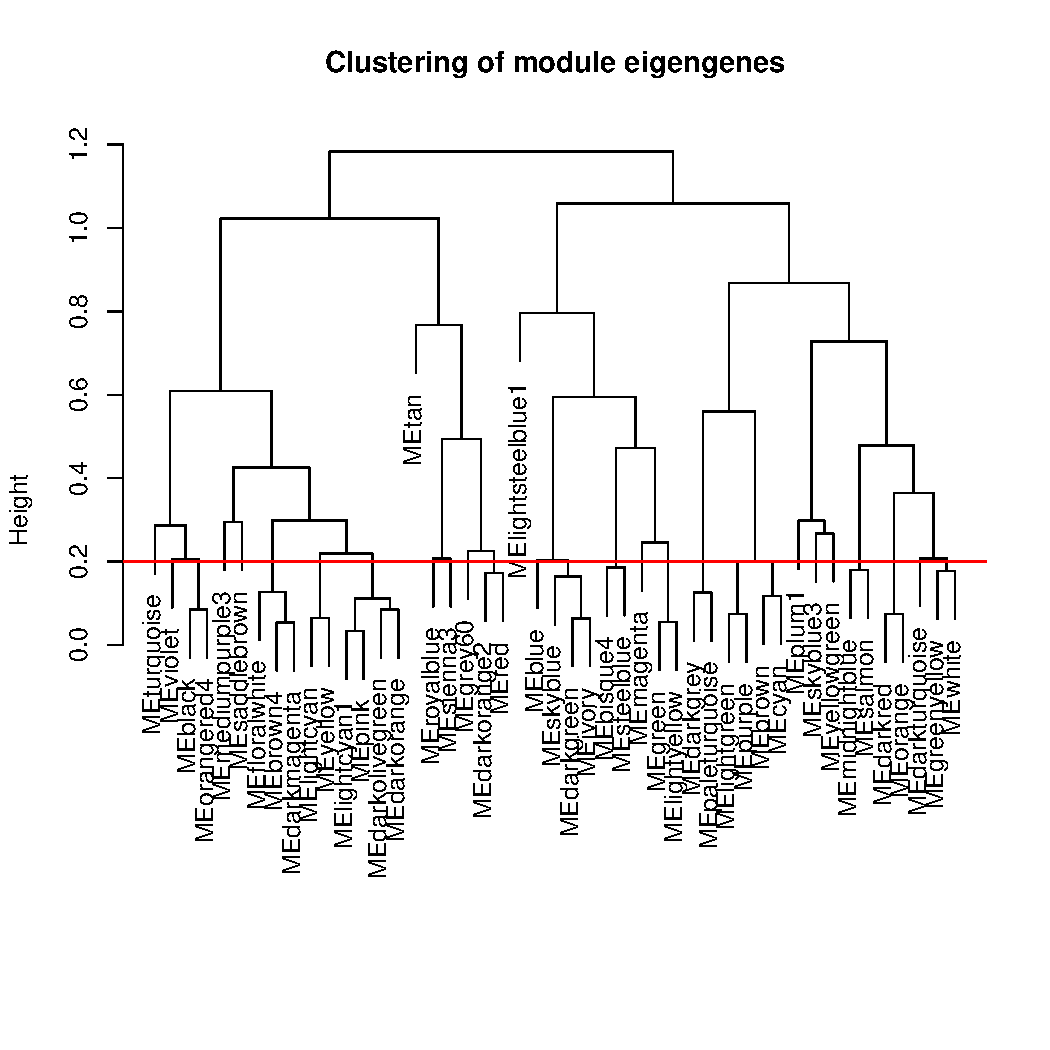
\includegraphics[width=\linewidth]{CapMergeLine}
    \caption{\textbf{Clustering of module eigengenes}}
    \label{fig:fsCLust}
\end{figure}


\begin{figure}[ht!]
      \centering
       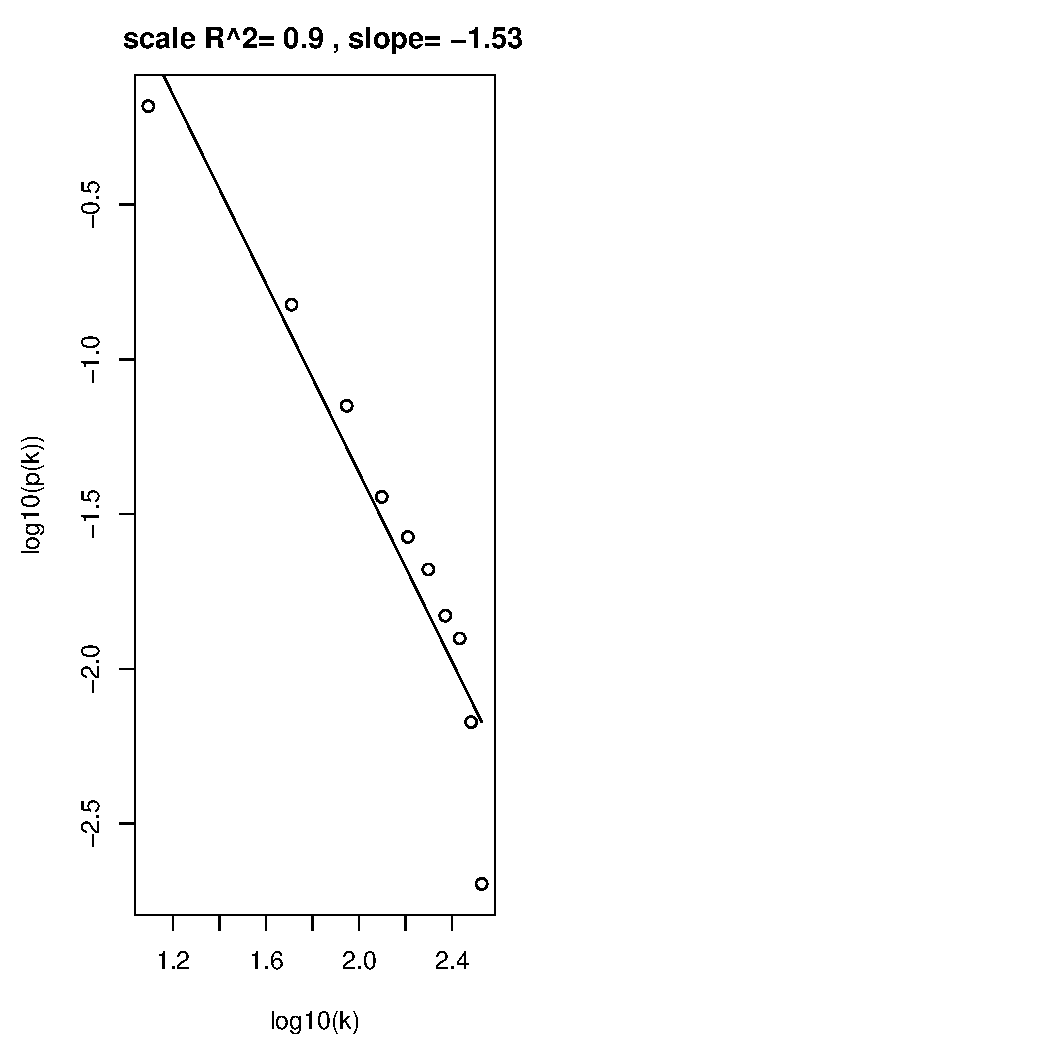
\includegraphics[width=\linewidth]{ScaleFree}
    \caption{\textbf{Coexpression modules are scale-free.} Genes were binned by connectivity level, k, and are plotted against the proportion of genes in each connectivity bin, p(k) on a log scale. R$^{2}$ = 0.9, slope = -1.53.}
    \label{fig:fsScale}
\end{figure}


\begin{figure}[ht!]
      \centering
       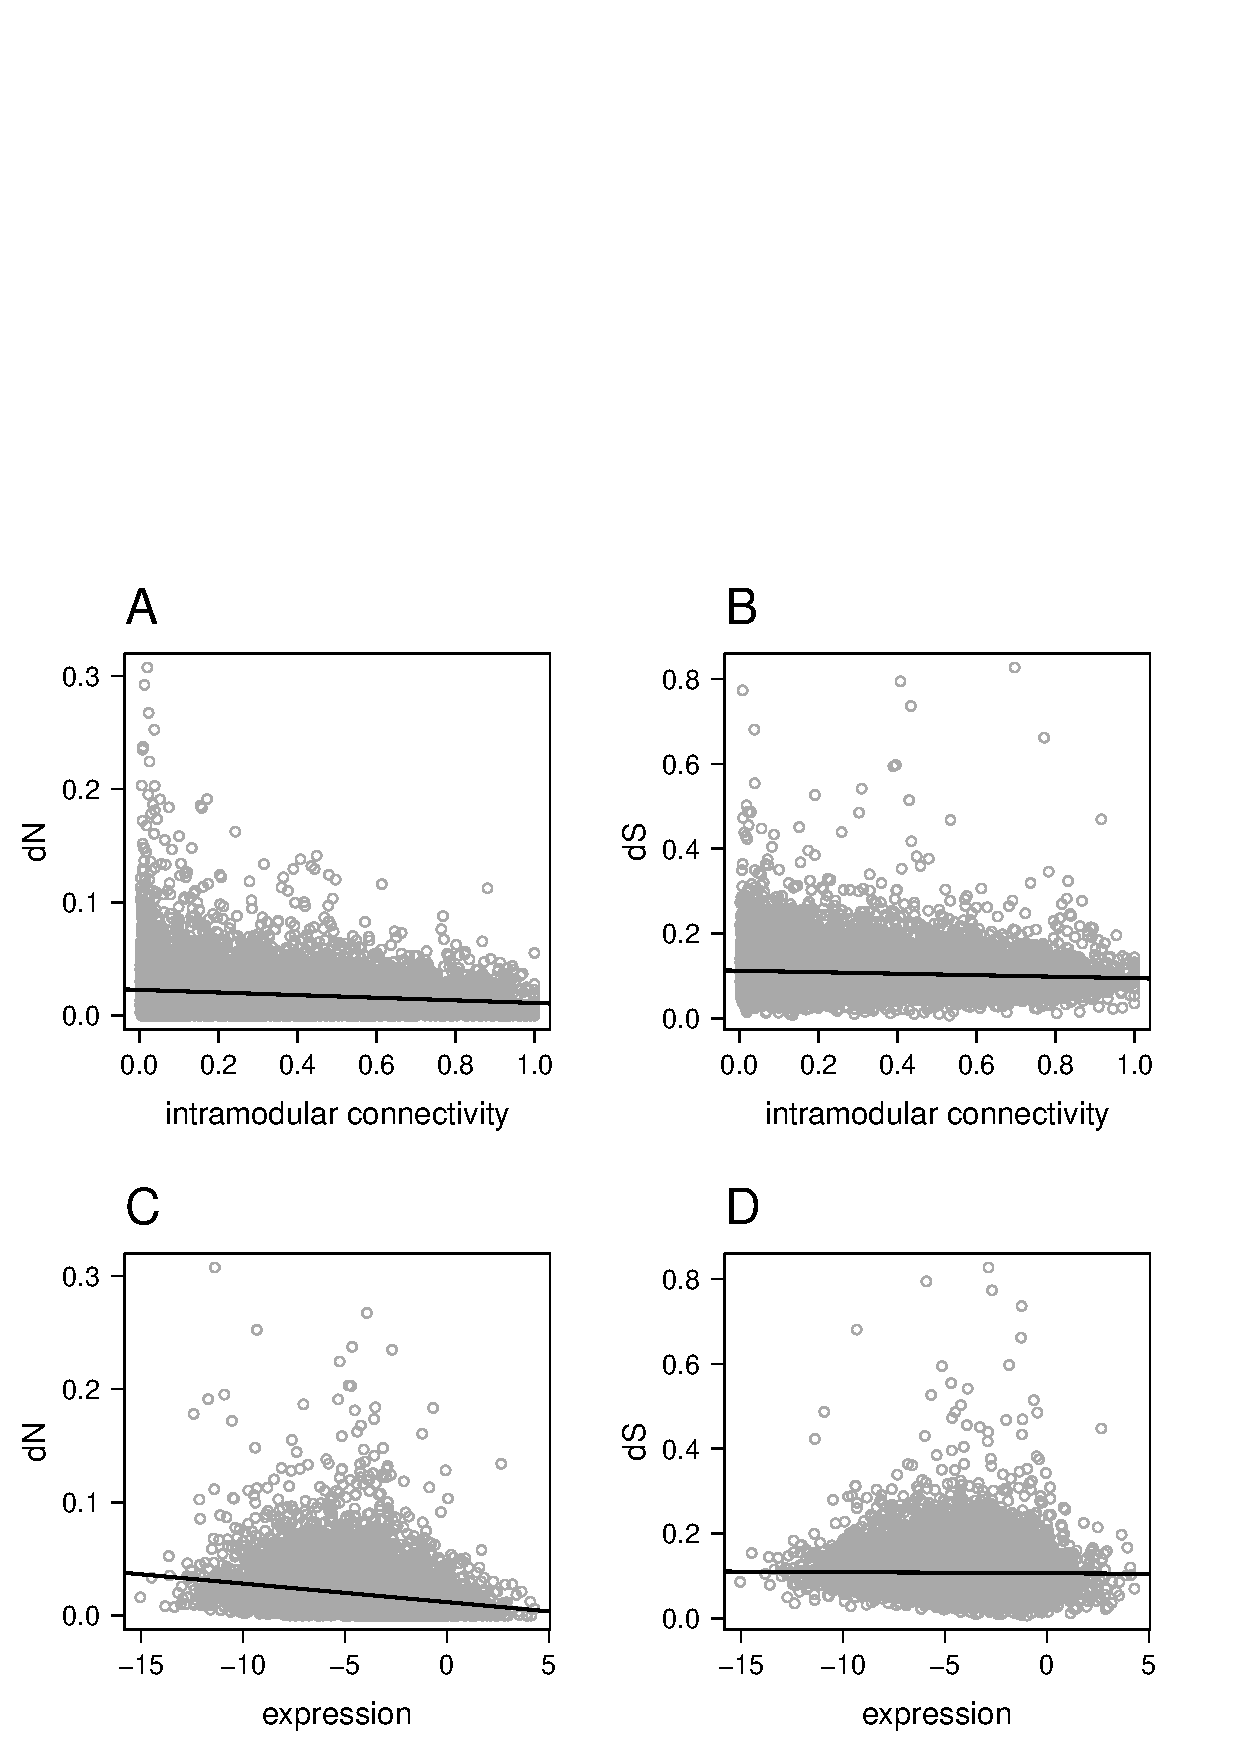
\includegraphics[width=\linewidth]{Ch4FigCorr}
    \caption{\textbf{Correlations between expression and intramodular connectivity and dN and dS.}}
    \label{fig:fsCorr}
\end{figure}


\begin{figure}[ht!]
      \centering
       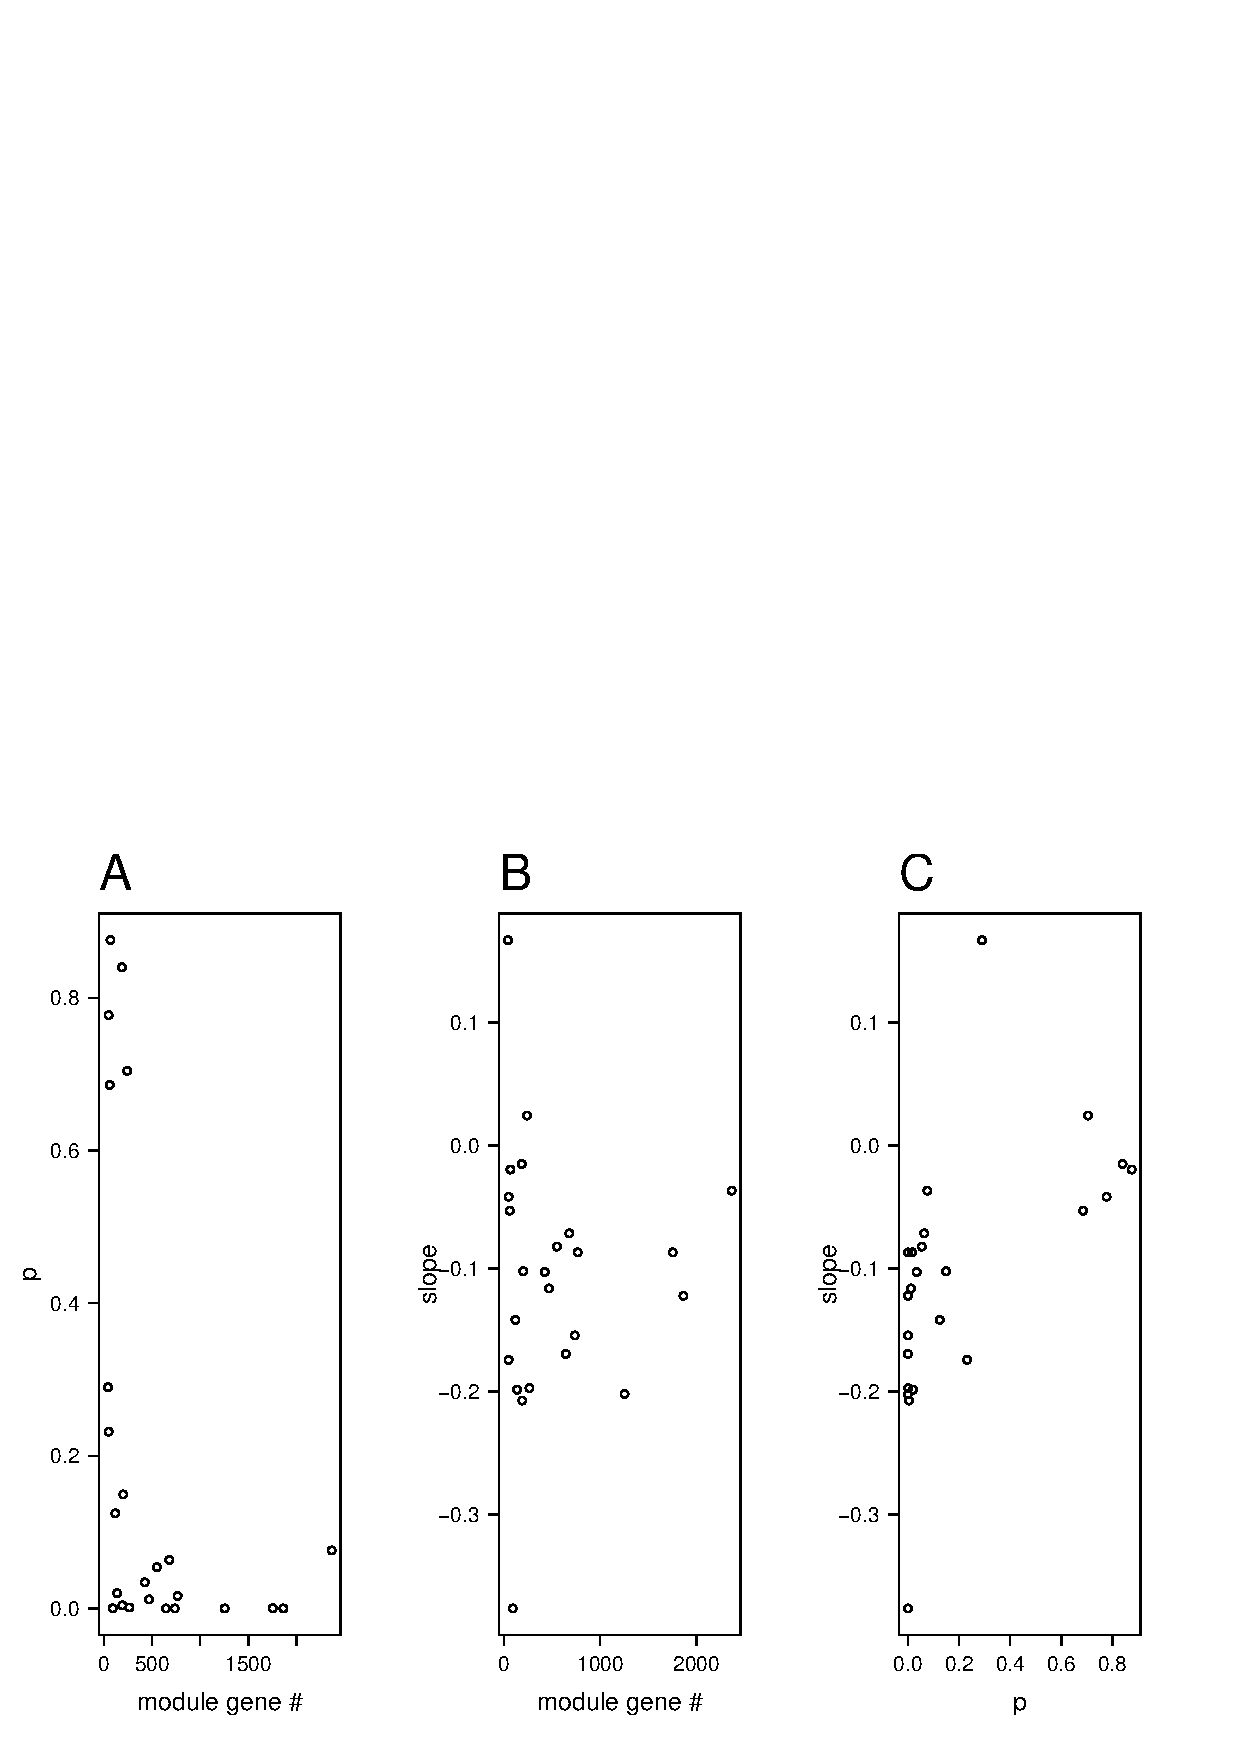
\includegraphics[width=\linewidth]{Ch4FigMod}
    \caption{\textbf{ Within-module estimates of the correlation between intramodular connectivity and dN/dS depend on module size}A) The number of genes in a module (x-axis) plotted against the p value for significance of the correlation between connectivity and dN/dS within that module (y-axis) B) THe number of genes in a module (x-axis) plotted against the slope of the relationship between connectivity and dN/dS (y-axis) C) The relationship between p (x-axis) and slope (y-axis) for within-module correlations of connectivity and dN/dS }
    \label{fig:fsMod}
\end{figure}




\begin{figure}[ht!]
      \centering
       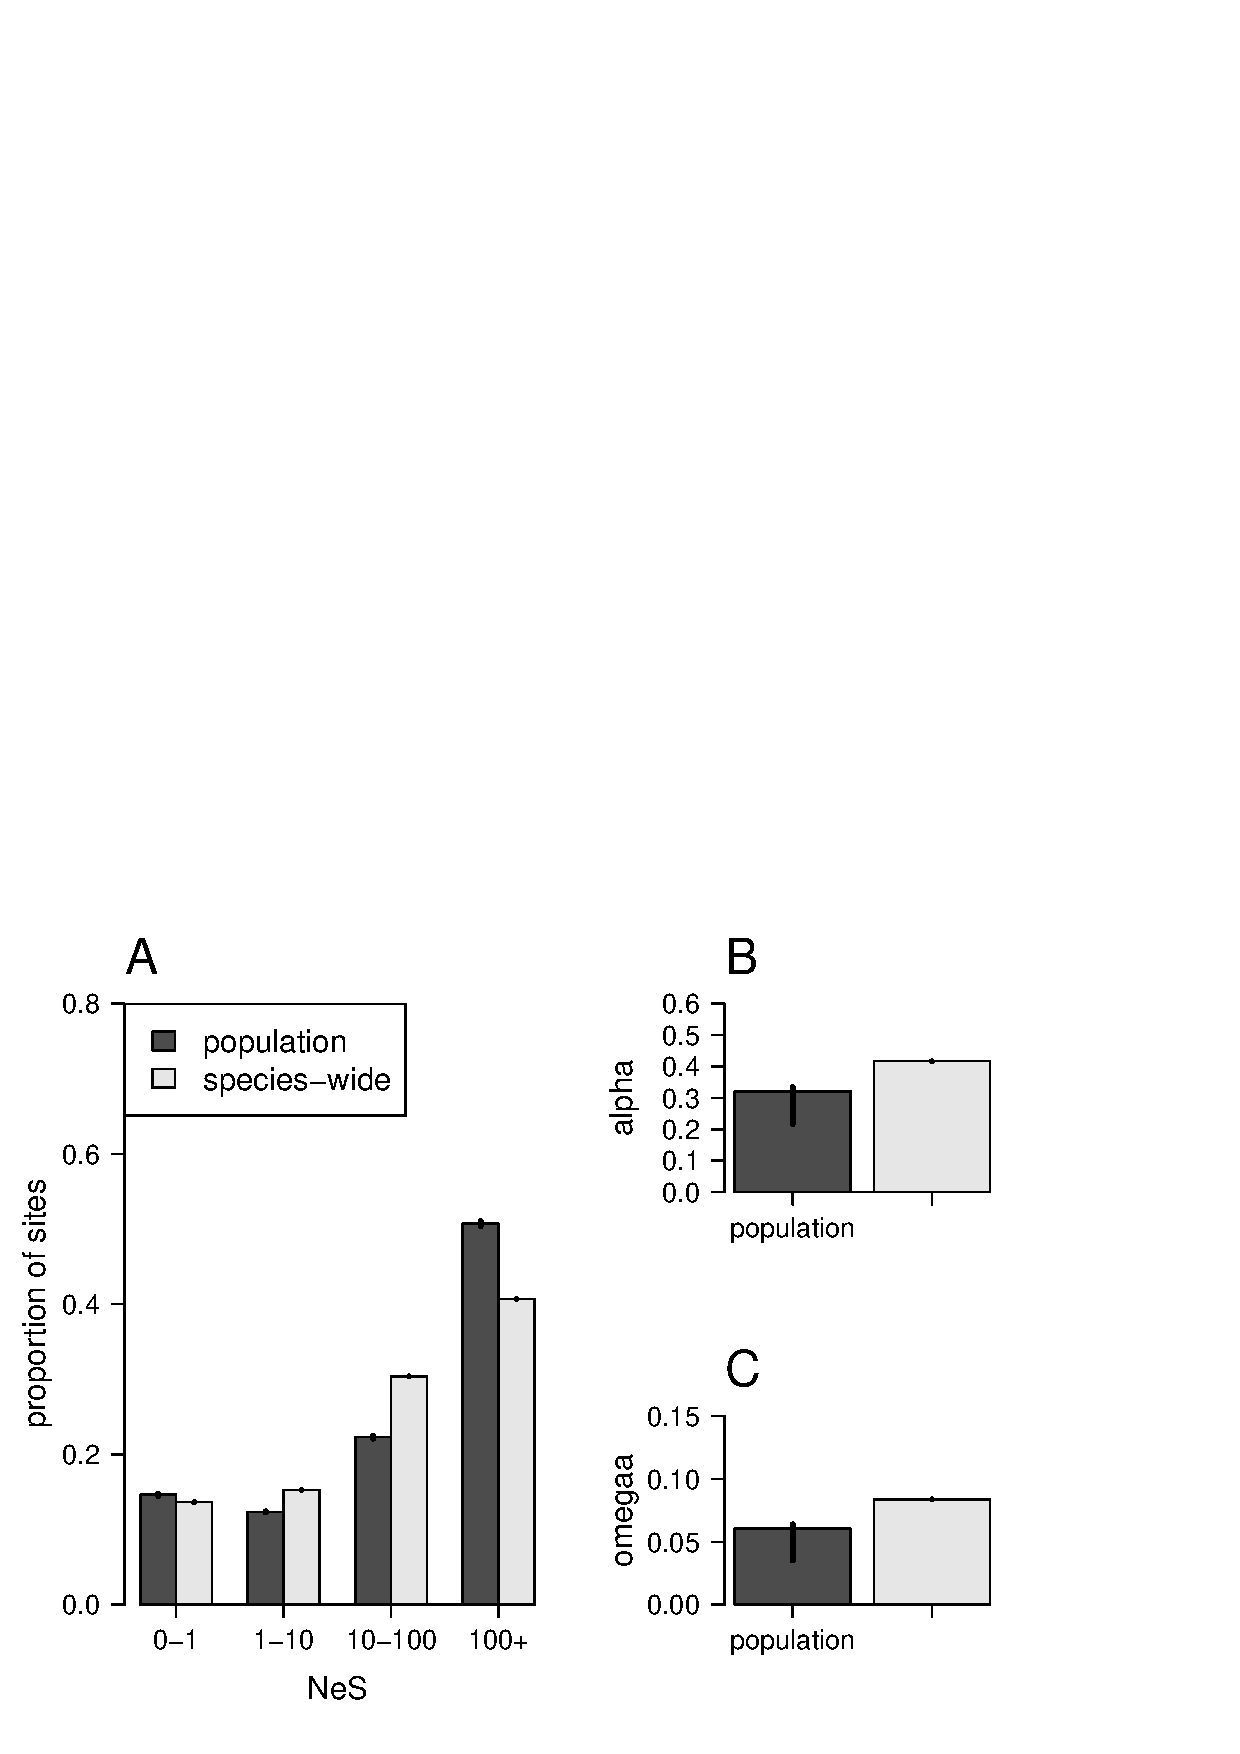
\includegraphics[width=\linewidth]{Ch4FigAll}
    \caption{\textbf{Positive and negative selection at 0-fold degenerate sites in all genes included in the coexpression analysis compared to selection on all 0-fold sites in a previously-reported species-wide sample.} A) The proportion of sites found in each bin of purifying selection strength. B) The proportion of sites fixed by positive selection, and C) the rate of adaptive substitution. Error bars represent 95\% confidence intervals and are only reported for the data from this study. Measurements of selection strength on the species-wide sample come from \citep{Williamson2014-tf}.}
    \label{fig:fsAll}
\end{figure}
